\section{Analisi del problema e Soluzioni}
In questa sezione verrà descritto il problema affrontato, le soluzioni scelte ed i rispettivi
risultati ottenuti.

\paragraph{Problema affrontato}
Il problema affrontato chiedeva di trovare pattern, anomalie e/o inferire sui dataset forniti, 
per ottenere, come risultato, informazioni su di essi mediante l'utilizzo di tecniche 
dell'analisi di serie temporali.

Per questioni di tempo il problema è stato ridotto all'analisi dei giunti del piede, più in particolare,
il tirocinio, è stato basato, sulla ricerca di uno o più metodi necessari a trovare la lunghezza di un passo
(stride) con successiva analisi dei risultati.



\paragraph{Risultati aspettati}
\begin{sloppypar}
Come risultati aspettati è stata presa in considerazione l'eventualità della non riuscita dell'obbiettivo finale,
quindi l'impossibilità di trovare, tramite le tecniche dell'analisi di serie temporali, una possibile soluzione
al problema.
\end{sloppypar}

In caso positivo, quindi di una possibile soluzione al problema posto, i risultati aspettati potrebbero essere:
\begin{itemize}
    \setlength\itemsep{-0.5em}
    \item Capacità da parte del metodo sviluppato di rilevare la durata del passo.
    \item Capacità da parte del metodo sviluppato di rilevare incorrettamente la durata del passo.
    \item Impossibilità da parte del metodo sviluppato di rilevare un passo.
\end{itemize}


\subsection{Prima soluzione}
In questa sezione verrà mostrata la prima soluzione al problema posto, nello specifico verrà
spiegata in breve l'idea generale, l'implementazione di alcuni dei metodi utilizzati, l'analisi dei
risultati, l'analisi della complessità ed infine le conclusioni.


\subsubsection{Idea generale}
L'idea generale, fulcro di questa soluzione, ruota intorno all'analisi della funzione di autocorrelazione.
Quest'ultima viene utilizzata per riconoscere pattern o una sorta di correlazione tra i dati non
visibile direttamente.

\subsubsection{Implementazione}
Mediante l'ausilio del test di Dickey-Fuller ed il calcolo della prima differenza è stato possibile
rendere le serie stazionarie, preparandole così alla successiva analisi di autocorrelazione.
\\
\paragraph*{Snippet} (\textit{Prima differenza})
\begin{minted}{python3}
    def compute_first_diff(series: list | np.ndarray):
        """ Calcola la prima differenza
        """
        
        if not isinstance(series, np.ndarray):
            series = np.array(series)

        return series[1:] - series[:len(series)-1]
\end{minted}

\paragraph*{Snippet} (\textit{Metodo per rendere la serie stazionaria})
\begin{minted}{python3}
    def make_stationary(series, max_steps = 30):
        """ Rende la serie stazionaria mediante il calcolo
            della prima differenza
        """
        step = 0   # numero di step
        s_copy = series.copy()  # copia della serie
        
        # fino a quando il test ritornca che la serie
        # non è stazionaria oppure sono stati superati
        # il massimo di step
        while(sts.adfuller(series)[1] > 0.05 
            and step < max_steps):
            
            # calcola la prima differenza
            serie = compute_first_diff(series)
            step += 1

        # se max_step è superato, non si è riusciti
        # a rendere la serie stazionaria
        if step > 30:
            series = s_copy

        return series
\end{minted}

\begin{sloppypar}
Avendo reso ogni serie stazionaria guardiamo alcuni dei grafici relativi all'autocorrelazione
di serie appartenenti a dataset dei soggetti $6$ ed $8$.
\end{sloppypar}

\begin{figure}[H]
    \centering
    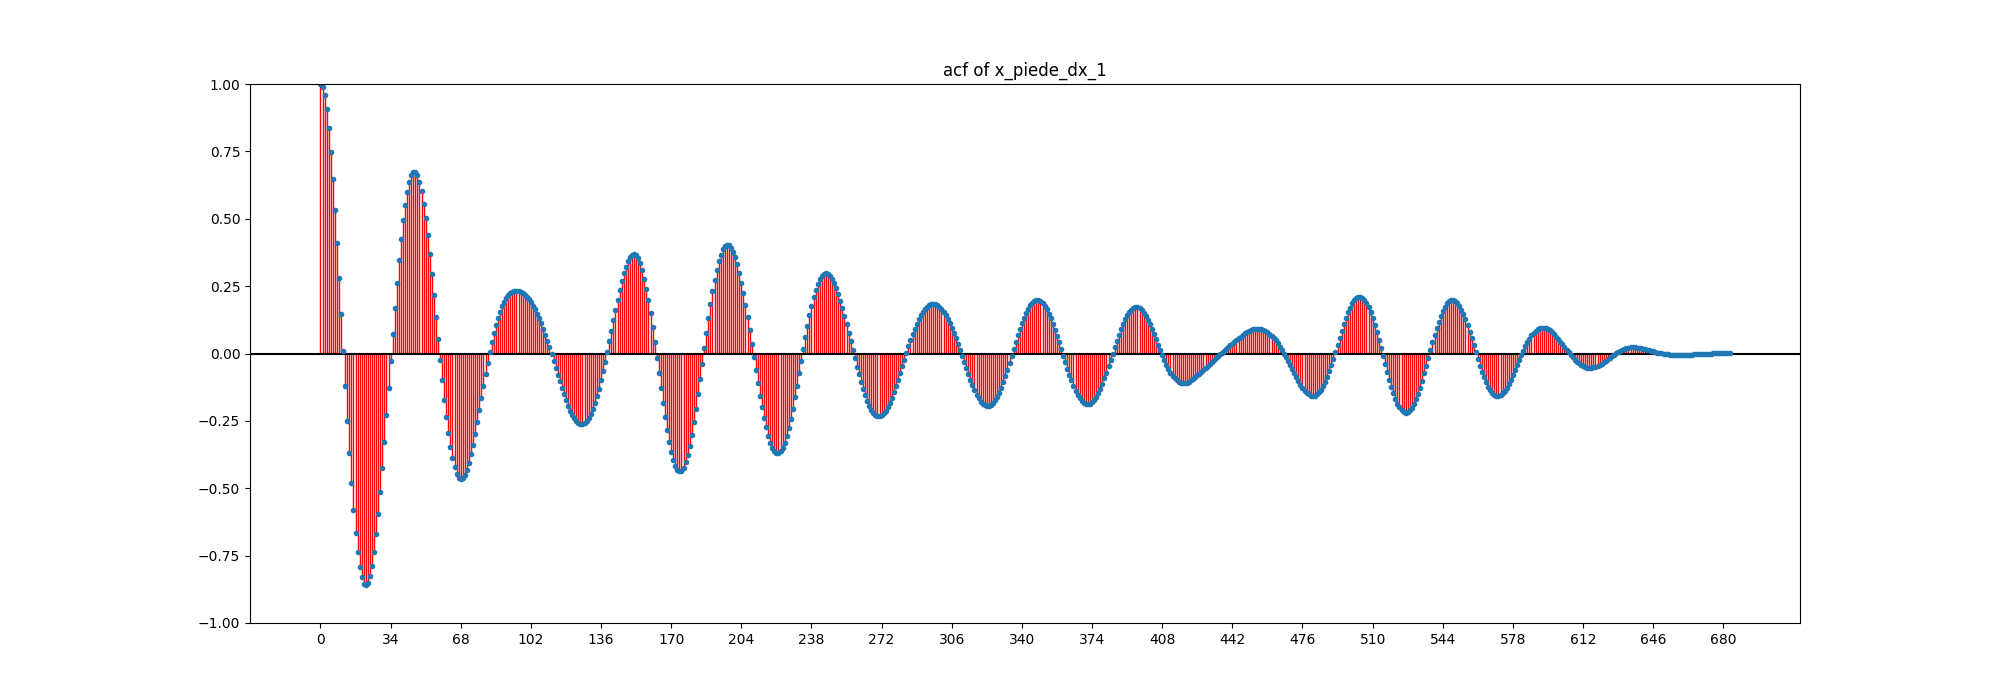
\includegraphics[width=\linewidth,keepaspectratio]{P006_x_piede_dx_1_acf.png}
    \caption{Soggetto $6$ autocorrelazione x piede destro posizione 1.}
    \label{fig:P006_x_piede_dx_1_acf}
\end{figure}

\begin{figure}[H]
    \centering
    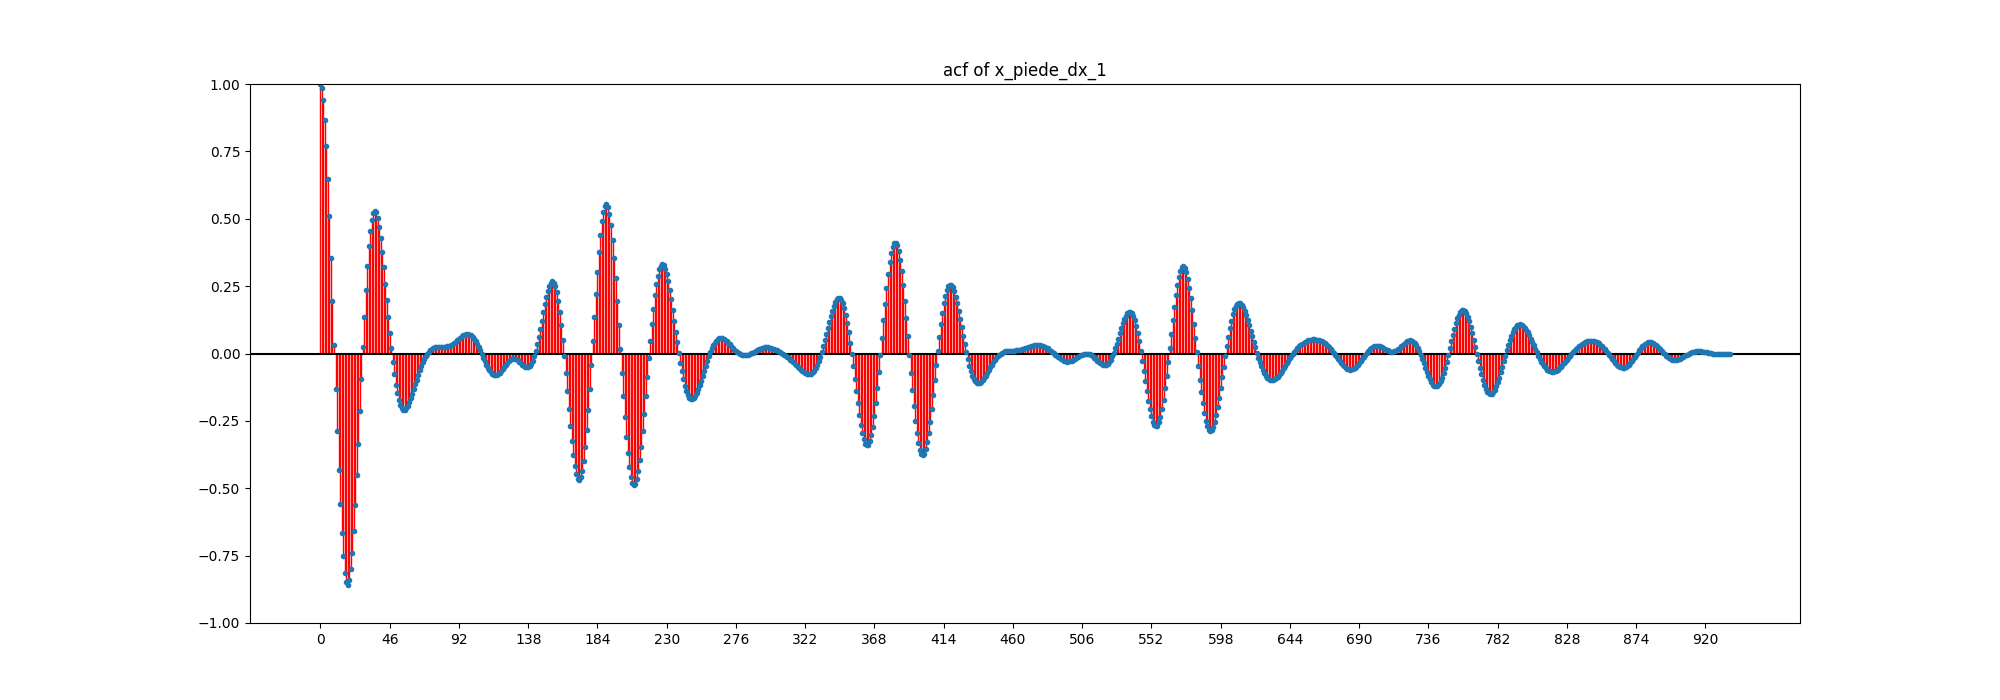
\includegraphics[width=\linewidth,keepaspectratio]{P008_x_piede_dx_1_acf.png}
    \caption{Soggetto $8$ autocorrelazione x piede destro posizione 1.}
    \label{fig:P008_x_piede_dx_1_acf}
\end{figure}

Da come si può notare dai grafici in figura~\ref{fig:P006_x_piede_dx_1_acf} e~\ref{fig:P008_x_piede_dx_1_acf}
l'autocorrelazione sembra riconoscere la durata di un passo in corrispondenza dei massimi locali.
\begin{sloppypar}
Utilizzando la funzione \texttt{argrelextrema} del modulo \texttt{statsmodels.tsa.stattools}
all'output della funzione di autocorrelazione è stato possibile recuperare gli argomenti (indici della lista) dei massimi locali.
Per esempio se prendiamo in considerazione il grafico~\ref{fig:P006_x_piede_dx_1_acf} gli argomenti
dei massimi locali sono
\end{sloppypar}
\[ [45, 95, 152, 197, 245, 297, 347, 395, 454, 504, 549, 592, 636, 678] \]
dove ogni argomento fa riferimento all'istante di tempo $t$, quindi al frame, in cui uno stride si ripete.

Questo ovviamente succede in linea teorica, non sempre è detto che il grafico dell'autocorrelazione
riesca ad ottenere con precisione quest'informazione, soprattutto se i dati non sono filtrati correttamente.

Continuado con l'implementazione del metodo, calcolando la distanza tra un argomento e l'altro troveremo
la durata di quel determinato passo. Prendendo sempre in considerazione la lista di agromenti sopra
e calcolandone la prima differenza otterremo
\[[50, 57, 45, 48, 52, 50, 48, 59, 50, 45, 43, 44, 42]\]
dove ogni elemento rappresenta la durata di un singolo stride.

Se calcoliamo la media otterremo la durata media di uno stride, che per la lista sopra sarà di 
$48.69\texttt{frame}$ cioè $1.623\texttt{secondi}$.

Questa serie di metodi è stata successivamente applicata ad ogni dataset ottenendo così la durata
media di uno stride per ogni posizione del piede destro e sinistro. Per fare ciò è stato creato
un ``mini'' programma che esegue automaticamente queste istruzioni ad ogni serie.

\subsubsection{Analisi dei risultati}
Analizzando i risultati soggetto per soggetto con camminata normale si è trovato che
i soggetti patologici hanno in media una durata di stride più elevata

\subsubsection{Analisi di complessità}
\subsubsection{Conclusioni}



\subsection{Seconda Soluzione}

\subsubsection{Idea generale}
\subsubsection{Implementazione}
\subsubsection{Analisi dei risultati}
\subsubsection{Analisi di complessità}
\subsubsection{Conclusioni}